\section{Results on the Benchmark}
\label{sec:results}
% SWEVO extension: the coefficient sweep (Fig. fig:S-csweep, Table tab:S-csweep), the PSO-dynamics diagnostic
% (Fig. fig:D-psodyn), the average ranks (Fig. fig:ranks), the wake loss versus N (Fig. fig:wakeloss), the equivalence
% curve (Fig. fig:equiv-curve) and the equivalence and heterogeneity tables (tab:X-equiv-levels, tab:X-heterogeneity)
% were moved here from the supplementary material (log: optA/sw/moved.md).
\makeatletter
% Capture the generated floats of the diagnostics and of the inference robustness checks; figures are stored like the
% tables (by their first \label) and placed with \swResFigure. The capture is global and typesets nothing.
\begingroup
\RenewEnviron{figure}[1][]{\supp@store}\RenewEnviron{figure*}[1][]{\supp@store}%
% [flattened: removed \CaptureSuppTables{analysis/mpce_supp_diag.tex}]
% [flattened: removed \CaptureSuppTables{analysis/mpce_supp_inference.tex}]
\endgroup
\newcommand{\swResFigure}[1]{\@ifundefined{supp@body@#1}{\par\noindent\TBD{generated figure \detokenize{#1} not found}\par}{%
  \@ifundefined{supp@used@#1}{\global\@namedef{supp@used@#1}{}%
    \begin{figure*}[!t]\@nameuse{supp@body@#1}\end{figure*}}{}}}
% Reference to a label that is either in the main text or (prefix S-) in the supplementary material: the generated
% captions use the supplement's label names; a label placed in the main text resolves there, any other one in the
% supplement (\swResRefs makes \ref behave like this inside a group). Aliases: supplement names of main-text labels.
\@namedef{swres@alias@prop:S-pso-stability}{prop:pso-stability}
\protected\def\swResRef#1{\@ifundefined{swres@alias@#1}%
  {\@ifundefined{r@#1}{\swres@origref{S-#1}}{\swres@origref{#1}}}%
  {\swres@origref{\@nameuse{swres@alias@#1}}}}
\let\swres@origref\ref
\newcommand{\swResRefs}{\let\ref\swResRef}
% generated full-width figures (csweep, diag_pso_dynamics) placed at 0.8\textwidth to save space
\newcommand{\swResNarrowGraphics}{\let\swres@ig\includegraphics
  \renewcommand{\includegraphics}[2][]{\swres@ig[width=0.8\textwidth]{##2}}}
% notes of tab:X-heterogeneity: long \multicolumn{8}{l} rows, set as wrapped paragraphs (as in the supplement)
\newcommand{\swResWrapNotes}{\let\swres@mc\multicolumn
  \def\multicolumn##1##2##3{\swres@mc{##1}{p{0.9\textwidth}}{##3}}}
% capture the floats (figures and tables) of a generated file without typesetting them
\newcommand{\swResCaptureFigs}[1]{\begingroup\RenewEnviron{figure}[1][]{\supp@store}\RenewEnviron{figure*}[1][]{\supp@store}%
  \CaptureSuppTables{#1}\endgroup}
\makeatother
This section reports the 68 benchmark cases (22{,}440 runs of 6,030 evaluations, random starts, 15$^\circ$ rose; per case: Tables~\ref{S-tab:res-1-500}--\ref{S-tab:res-2-1000}).

\subsection{Effect of the Baseline Setting}
\label{sec:psosetting}
\label{sec:baseline}
% >>>>> begin analysis/mpce_tab_baseline.tex
%% generated by mpce_results.py -- do not edit by hand
\begin{table}[!t]
\centering
\caption{Effect of the PSO setting on an eight-method pool (the methods of Table~\ref{tab:friedman68} with LX-SSA-VNS instead of PSO-VNS; 68 cases, 6,030 evaluations).}
\label{tab:baseline}
\footnotesize\setlength{\tabcolsep}{4pt}
\begin{tabular}{lcc}
\toprule
& \multicolumn{2}{c}{PSO setting} \\
\cmidrule(lr){2-3}
Method & Old & Constriction \\
\midrule
LX-SSA-VNS & 2.65 & 3.41 \\
SSA-VNS & \textbf{1.99} & 2.77 \\
LX-SSA & 5.65 & 6.06 \\
SSA & 4.81 & 5.34 \\
PSO & 5.04 & \textbf{1.53} \\
DE & 6.99 & 7.03 \\
VNS & 3.59 & 4.15 \\
MS-SLSQP & 5.28 & 5.71 \\
\midrule
PSO position & 5 & 1 \\
LX-SSA-VNS vs.\ PSO (W/T/L) & 35/33/0 & 0/21/47 \\
SSA-VNS vs.\ PSO (W/T/L) & 41/27/0 & 0/22/46 \\
\bottomrule
\multicolumn{3}{p{0.95\columnwidth}}{Old: $w=0.7$, $c_1=c_2=2$; constriction: Clerc--Kennedy setting~\cite{Clerc2002}. Average rank: 1 = best, feasibility-aware rule (fewer than 15 of 30 feasible runs in a case = ranked below the qualified methods); bold: best average rank. W/T/L: cases in which the hybrid is significantly better / not different / worse than PSO (two-sided Wilcoxon signed-rank test, 30 seed-paired runs, Holm-adjusted over the seven comparisons of the hybrid in each case, $\alpha=0.05$).}
\end{tabular}
\end{table}
% <<<<< end analysis/mpce_tab_baseline.tex
The old setting lies beyond the order-2 (variance) stability boundary~\eqref{eq:poli}. Run on the same cases, budget and seeds as the constriction setting~\eqref{eq:constriction}, it returns a feasible layout in only 86.0\% of the runs (fewer than 15 feasible runs in 8 cases), is significantly worse in 56 of the 68 cases and never better, and has a mean wake loss 0.61~pp higher over the 60 cases in which both settings have at least 15 feasible runs.
% CHECK-FINAL [C12]: pso_setting: constriction_vs_old L == 0, W >= 34 (editor cut C5 applied)

% Page budget: kept in the supplementary material: \swResFigure{fig:D-psodyn}
\emph{What goes wrong.} In instrumented reruns (clipping without velocity reset or clamping; Fig.~\ref{S-fig:D-psodyn} and Table~\ref{S-tab:D-psodyn}), its swarm contracts much less (final spread 8.9 times, velocity 13 times that of the constriction setting), 8.7\% of the coordinates are clipped (constriction: 1.6\%), and far fewer particle evaluations in the second half of a run are feasible (2.6\% vs.\ 48.4\%). With the constriction setting the spread around $\mathbf G$ shrinks steadily, as expected under order-2 stability (limit variance $\propto(P^i_m-G_m)^2$; Proposition~\ref{prop:pso-stability}); with the old setting it stays at a sizeable fraction of the radius, the large steps keep pushing coordinates onto the box, where a clipped coordinate stays while its kept velocity points outward and violates the circular boundary (Lemma~\ref{S-lem:S-clip}), and most infeasible evaluations violate both constraints.
% CHECK-DIAG [D03] spread/|V| ratios ("contracts much less"); [D04] clipped share; [D05] feasible particle evaluations (iterations 101-200); [D07] most infeasible particle evaluations of the old setting violate both constraints; [D01] instrumented runs reproduce the stored runs

The \emph{final} layouts, in contrast, mostly violate only the spacing (224 of 286; boundary only 10, both 52; constriction: none), an effect of the penalty scaling in~\eqref{eq:penalty} ($g^{\rm b}_i$ in m$^2$, $g^{\rm s}_{ij}$ in m): the best infeasible layout lies inside the circle with turbines slightly too close, and 60 of the 62 boundary violations are turbines pinned at the box near a tangent point, where $g^{\rm b}_i$ is cheap (Section~\ref{sec:constraints}).
% CHECK-DIAG [D06] infeasible finals of the old setting mostly spacing-only (224 of 286), boundary-only < spacing-only, constriction none; [D21] >= 90 % of boundary-violating finals pinned at the box (tangent point)

% Page budget: only the figure of analysis/mpce_supp_csweep.tex is placed; its table stays in the supplementary material
% [flattened: removed \swResCaptureFigs{analysis/mpce_supp_csweep.tex}]
\begingroup\swResRefs\swResNarrowGraphics%
% --- float fig:S-csweep from analysis/mpce_supp_csweep.tex
\begin{figure*}[!t]
\centering
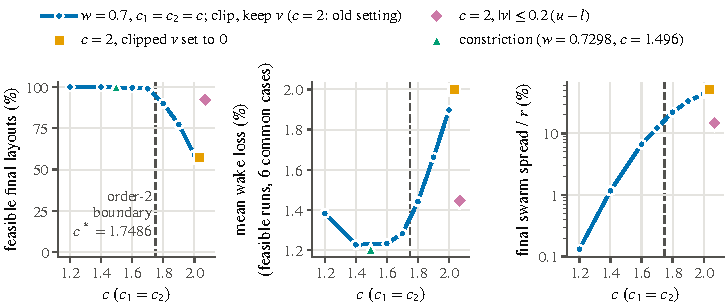
\includegraphics[width=\textwidth]{figures_mpce/csweep.pdf}
\caption{Stand-alone PSO with $w=0.7$ and $c_1=c_2=c$ on the 12 split cases $\times$ 30 seeds (6{,}030 evaluations, random starts; line with circles), the old setting ($c=2$) with two other bound-handling rules (clipped velocity components set to zero; velocity clamping $|v|\le v_{\max}=0.2\,(u-l)$; drawn slightly to the right of $c=2$), and the constriction setting ($w=0.7298$, $c=1.49618$; stored runs of the main comparison, spread not logged). The dashed vertical line is the order-2 stability boundary $c^\ast=12(1-w^2)/(7-5w)=1.7486$ of Proposition~\ref{prop:S-pso-stability} (stagnation, no bounds). Left: feasible final layouts (\% of 360 runs). Middle: mean wake loss of the feasible runs, averaged over the 6 cases in which every setting has at least 15 feasible runs. Right: median final swarm spread (mean over particles of the RMS turbine distance to the global best), relative to the farm radius (log scale). All settings start from the same seeded initial swarm. Values: Table~\ref{tab:S-csweep}.}
\label{fig:S-csweep}
\end{figure*}
\endgroup
\emph{Coefficient sweep.} A sweep of $c_1=c_2=c$ at $w=0.7$ (Fig.~\ref{fig:S-csweep} and Table~\ref{S-tab:S-csweep}; 360 runs per setting; $c=2.0$ reproduces the stored old-setting runs bit for bit) shows that the boundary $c^\ast=1.7486$ marks approximately where this PSO starts to fail: at least 98.9\% of the runs are feasible for $c\le1.7$, then feasibility declines progressively (90.0\% at $c=1.8$, 58.9\% at 2.0); velocity clamping raises it to 92.2\%, still worse than constriction in all 12 cases.
% CHECK-CSWEEP [S01] c = 2.0 reproduces the stored old-setting runs; [S02] c <= 1.7 >= 98 % feasible; [S03] c = 1.8 > 1.9 > 2.0; [S04] decline starts in the step containing c*; [S05] progressive, no jump; [S10] vmax >= 90 %; [S11] vmax worse than constriction in all 12 cases (never "causes")
There is no step at $c^\ast$: the decline begins between 1.7 and 1.8 and accelerates, while the swarm spread grows smoothly with $c$ (by about an order of magnitude from $c=1.4$ to 1.7) and the wake loss rises already on the stable side (lower at $c=1.6$ than at 1.7 in 10 of 12 cases, $p=0.005$), then in all 12 cases from 1.7 to 1.8. The boundary marks where the steps become too large for this bounded problem; the sweep does not show that crossing it causes the failure.
% CHECK-CSWEEP [S06] spread grows monotonically, >= 5x from 1.4 to 1.7; [S07] loss degrades on the stable side, c = 1.6 beats 1.7 in >= 10 of 12 (Wilcoxon p < 0.05); [S08] 1.7 -> 1.8 worsens the loss in all 12 cases
Zeroing clipped velocity components does not rescue the old setting (57.2\% feasible), whereas clamping brings it to about the level of $c=1.8$: the deficit comes mainly from the large steps, not from the bound handling.
% CHECK-CSWEEP [S09] zeroing clipped velocities no rescue; [S12] vmax indistinguishable from c = 1.8

Table~\ref{tab:baseline} shows the effect on a comparison. It ranks an eight-method pool, the methods of Table~\ref{tab:friedman68} with LX-SSA-VNS instead of PSO-VNS, once with each PSO setting (all other methods use identical runs): with the old setting, SSA-VNS ranks first and PSO only in position 5, behind both salp-swarm hybrids; with the constriction setting, PSO ranks first, ahead of every salp-swarm method (standard coefficients~\cite{Clerc2002}; none of the methods was tuned on these cases). The reversal holds at 6,030 evaluations; on the six largest cases at 120,030, SSA-VNS ranks ahead of PSO (4.17 vs.\ 5.83; Section~\ref{sec:budget}). The old setting thus makes the methods compared with it, including LX-SSA~\cite{Solanki2023}, appear stronger than they are.
% CHECK-FINAL [C27]: same pool: old setting SSA-VNS (1.99) and LX-SSA-VNS (2.65) ahead of PSO (5.04, NBaseOldPSOPos); constriction PSO ahead of every salp-swarm method (NBaseNewBest = PSO)
% CHECK-FINAL [C45]: at 120,030 evaluations SSA-VNS ranks ahead of PSO on the six largest cases

\subsection{Overall Comparison}
\label{sec:overall}
% >>>>> begin analysis/mpce_tab_friedman68.tex
%% generated by mpce_results.py -- do not edit by hand
\begin{table}[!t]
\centering
\caption{Case-level analysis of the eight methods over the 68 benchmark cases.}
\label{tab:friedman68}
\scriptsize\setlength{\tabcolsep}{2pt}
\begin{tabular}{lcccccc}
\toprule
Method & Avg.\ rank & Best & Feas. & $p_z$ & $p_W$ & $\overline{\Delta L}$ \\
\midrule
PSO-VNS & 1.82 & 29 & 100.0 & -- & -- & -- \\
PSO & 1.97 & 25 & 100.0 & 0.713 & 0.296 & $-0.018$ \\
SSA-VNS & 3.45 & 0 & 99.6 & $2.0\times10^{-4}$ & $5.7\times10^{-11}$ & $-0.330$ \\
VNS & 4.40 & 3 & 100.0 & $2.4\times10^{-9}$ & $1.3\times10^{-10}$ & $-0.465$ \\
SSA & 5.38 & 0 & 97.6 & $8.3\times10^{-17}$ & $4.5\times10^{-11}$ & $-0.611$ \\
MS-SLSQP & 5.88 & 1 & 100.0 & $1.8\times10^{-21}$ & $4.2\times10^{-11}$ & $-0.435$ \\
LX-SSA & 6.06 & 0 & 96.9 & $3.3\times10^{-23}$ & $4.5\times10^{-11}$ & $-0.765$ \\
DE & 7.04 & 0 & 71.4 & $1.0\times10^{-34}$ & $5.6\times10^{-11}$ & $-0.887$ \\
\bottomrule
\end{tabular}
\par\vspace{2pt}\parbox{\columnwidth}{\scriptsize Avg.\ rank: average rank of the mean feasible objective, i.e., conditional quality subject to qualification, not reliability (1 = best; fewer than 15 feasible runs in a case = ranked below the qualified methods, by number of feasible runs); Best: cases in which the method alone ranks first; Feas.: feasible runs (\%); $p_z$: Holm-adjusted $p$ of the average-rank test against PSO-VNS. Because mean-rank tests depend on the pool~\cite{Benavoli2016}, $p_W$ gives the two-sided Wilcoxon signed-rank test on the 68 per-case mean wake losses (Holm-adjusted over the 7 methods) and $\overline{\Delta L}$ the mean wake-loss difference (pp, PSO-VNS minus method; negative = PSO-VNS better) over the cases in which both methods have at least 15 feasible runs (66 for SSA, 66 for LX-SSA, 50 for DE, otherwise 68). Friedman $\chi^2_F=319.3$ (7 d.f.), $p=4.6\times10^{-65}$; Iman--Davenport $F_F=136.5$ (7, 469 d.f.), $p=6.7\times10^{-109}$.}
\end{table}
% <<<<< end analysis/mpce_tab_friedman68.tex
% >>>>> begin analysis/mpce_tab_wtl.tex
%% generated by mpce_results.py -- do not edit by hand
\begin{table}[!t]
\centering
\caption{Run-level outcome of PSO-VNS against each method (W/T/L over the 68 cases).}
\label{tab:wtl}
\scriptsize\setlength{\tabcolsep}{1.6pt}
\begin{tabular}{llcccccccc}
\toprule
DS & $r$ (m) & Cases & PSO & \begin{tabular}{@{}c@{}}SSA-\\VNS\end{tabular} & SSA & \begin{tabular}{@{}c@{}}LX-\\SSA\end{tabular} & DE & VNS & \begin{tabular}{@{}c@{}}MS-\\SLSQP\end{tabular} \\
\midrule
I & 500 & 9 & 0/8/1 & 6/3/0 & 8/1/0 & 8/1/0 & 7/2/0 & 6/3/0 & 7/2/0 \\
I & 750 & 11 & 1/8/2 & 9/2/0 & 10/1/0 & 10/1/0 & 9/2/0 & 8/3/0 & 10/1/0 \\
I & 1000 & 14 & 3/11/0 & 9/5/0 & 12/2/0 & 12/2/0 & 12/2/0 & 12/2/0 & 12/2/0 \\
II & 500 & 9 & 3/5/1 & 7/2/0 & 7/2/0 & 8/1/0 & 7/2/0 & 7/1/1 & 8/1/0 \\
II & 750 & 11 & 2/9/0 & 8/3/0 & 10/1/0 & 10/1/0 & 9/2/0 & 8/3/0 & 9/2/0 \\
II & 1000 & 14 & 5/9/0 & 10/4/0 & 12/2/0 & 12/2/0 & 12/2/0 & 10/4/0 & 13/1/0 \\
\midrule
All & & 68 & 14/50/4 & 49/19/0 & 59/9/0 & 60/8/0 & 56/12/0 & 51/16/1 & 59/9/0 \\
$\tilde r_{\rm rb}$ & & & +0.08 & +0.72 & +0.98 & +0.97 & +1.00 & +0.84 & +0.99 \\
\bottomrule
\end{tabular}
\par\vspace{2pt}\parbox{\columnwidth}{\scriptsize W/T/L: cases in which PSO-VNS is significantly better / not different / worse (two-sided Wilcoxon signed-rank test on 30 seed-paired runs, $\alpha=0.05$, Holm-adjusted over the seven comparisons of PSO-VNS in each case, a different family from Table~\ref{tab:ablation}; an infeasible run ranks below every feasible run). $\tilde r_{\rm rb}$: median rank-biserial correlation (positive = PSO-VNS better; zero differences dropped, $r_{\rm rb}=0$ if all are zero).}
\end{table}
% <<<<< end analysis/mpce_tab_wtl.tex

\begin{table}[!t]
\centering\footnotesize
\caption{Expanded nine-method benchmark pool. Original eight-method results remain a separate analysis.}
\label{tab:ga-main}
\begin{tabular}{lcccc}\toprule
Method & Avg. rank & Best & Feas. (\%) & $p_W$ vs. GA \\\midrule
PSO-VNS & \textbf{2.18} & \textbf{21} & 100.0 & 0.101 \\
PSO & 2.40 & 17 & 100.0 & 0.696 \\
GA & 2.74 & 16 & 98.6 & -- \\
SSA-VNS & 4.32 & 0 & 99.6 & $9.29\times10^{-10}$ \\
VNS & 5.21 & 3 & 100.0 & $1.07\times10^{-9}$ \\
SSA & 6.34 & 0 & 97.6 & $6.06\times10^{-11}$ \\
MS-SLSQP & 6.85 & 1 & 100.0 & $2.34\times10^{-10}$ \\
LX-SSA & 7.01 & 0 & 96.9 & $6.06\times10^{-11}$ \\
DE & 7.96 & 0 & 71.4 & $1.14\times10^{-10}$ \\
\bottomrule\end{tabular}
\par\vspace{3pt}\parbox{\linewidth}{\footnotesize 68 cases, 30 paired seeds, 6,030 evaluations. Best: cases won outright; bold: best method. $p_W$: Holm-adjusted case-mean Wilcoxon comparison with GA. Qualification and conditional quality follow Section~\ref{sec:setup-stats}; ranks depend on the method pool. Source: Table~\ref{S-tab:S-rev-ga}.}
\end{table}

Over the eight methods (Table~\ref{tab:friedman68}), the Friedman test rejects the hypothesis of equal performance ($\chi^2_F=319.3$, $p=\ensuremath {4.6\times 10^{-65}}$; Iman--Davenport $F_F=136.5$, $p=\ensuremath {6.7\times 10^{-109}}$). PSO-VNS has the best average rank (1.82), alone ranks first in 29 cases, and stays first when the final layouts are re-evaluated with 5$^\circ$ or 1$^\circ$ direction sub-bins (1$^\circ$: 2.09; Section~\ref{sec:robustness}). In the Holm-adjusted post hoc tests ($p_z$ in Table~\ref{tab:friedman68}; tied ranks make them conservative), PSO-VNS ranks significantly better than SSA-VNS, VNS, SSA, MS-SLSQP, LX-SSA and DE, but not than PSO ($p_{\rm Holm}=0.71$). The rank order and these conclusions are unchanged for thresholds of 1, 10, 15, 20, 25 and 30 feasible runs; significant comparisons with PSO-VNS favor the same method in each of the six clusters, and leaving out one cluster changes none of them (Tables~\ref{S-tab:X-threshold}--\ref{S-tab:X-loco}). The real-coded GA (Section~\ref{sec:setup-cases}) does not change this picture (Table~\ref{tab:ga-main}; details: Table~\ref{S-tab:S-rev-ga}): in the nine-method pool it ranks third (2.74, against 2.18 for PSO-VNS and 2.40 for PSO; Holm $p=0.47$ against either), and it is practically equivalent to PSO at the case level (GA $-$ PSO: $+0.008$~pp, 90\% CI [$-$0.022, 0.041]), whereas its interval against PSO-VNS, [$-$0.006, 0.062]~pp, extends beyond the margin. Its leads at the sites are reported in Sections~\ref{sec:hornsrev-site} and~\ref{sec:iea37}.
% CHECK-FINAL [C01]: main.friedman.best_ranked == PSOBV; [C02]: p < 0.05 (verb generated: \NFriedVerb); [C03]: p_holm_vs_focus: only PSOC >= 0.05
% CHECK-DIR [F06]: PSO-VNS best average rank with 5-deg and 1-deg sub-bins (\NFRankPSOVNSOne)
% CHECK-EXTRA [X02][X03][X05]-[X09] six thresholds 1-30; [X11] clusters 6/6 same direction for comparisons with PSO-VNS; [X14] LOCO changes only \NXLocoChanged (not a PSO-VNS comparison), PSO-VNS always best

% Page budget: the rank chart stays in the supplementary material (Fig. S-fig:S-ranks); the main-text version was:
% \begin{figure}[!t]
% \centering
% \pipefig{0.4\textwidth}{figures_mpce/avg_ranks.pdf}{5cm}
% \caption{Average rank of the eight methods of the main comparison over the 68 benchmark cases (feasibility-aware ranking of Table~\ref{tab:friedman68}; 1 = best).}
% \label{fig:ranks}
% \end{figure}
% CHECK (pipeline): avg_ranks.pdf is drawn from the same ranks as tab:friedman68 (\NRankPSOVNS ... \NRankDE)
In Fig.~\ref{S-fig:S-ranks}, the two PSO-based methods lead with a small gap, far ahead of SSA-VNS; both hybrids rank ahead of their first phase and of VNS, and the last rank of DE also reflects its feasibility (71.4\% of its runs). Figs.~\ref{S-fig:S-box-max} and~\ref{S-fig:S-box-mid} show the distributions of the feasible runs for the largest and the middle $N$ of each farm.
% CHECK (pipeline): rank values from tab:friedman68; [C01] PSO-VNS best; DE feasibility \NFeasDE (CHECK-FINAL [C08])

Against SSA-VNS, PSO-VNS is significantly better in 49 cases and never worse ($p_{\rm Holm}=\ensuremath {5.7\times 10^{-11}}$). Against SSA, LX-SSA, DE, VNS and MS-SLSQP (untuned DE; finite-difference gradients), it is significantly better in most cases; it is never significantly worse than SSA-VNS, SSA, LX-SSA, DE and MS-SLSQP and significantly worse than VNS in one case. On the all-run paired outcome, too, PSO-VNS is better than each of these six methods (Section~\ref{sec:archive-reliability}). PSO-VNS is more reliable in reaching feasibility on the Horns Rev~1 block with random starts (30/30 vs.\ 19/30, McNemar $p=\ensuremath {9.8\times 10^{-4}}$; Section~\ref{sec:hornsrev-site}) and ranks best on the six largest cases at all three budgets (exploratory; Section~\ref{sec:budget}). The leading methods depend on the conditions: from feasible starts, VNS ranks first (Section~\ref{sec:feasinit}); under the Gaussian wake, PSO ranks narrowly ahead of PSO-VNS with 15$^\circ$ bins but not with 1$^\circ$ sub-bins (Section~\ref{sec:gaussian}).
% CHECK (manual, 2026-10-04): all-run scores of PSO-VNS 0.734 (SSA-VNS) ... 0.897 (DE), case CIs lower limits >= 0.700 (analysis/rev3_inference.json, tab:S-r3-allrun); order by score SSA-VNS, VNS, MS-SLSQP, SSA, LX-SSA, DE
% CHECK-FINAL [C06]: wtl.SSABV.L == 0; [C07]: better than SSA, LX-SSA, DE, VNS, MS-SLSQP in most cases; [C08]/[C20]: Horns Rev PSO-VNS 30/30, PSO < 30/30; [C29]: six largest cases best at all budgets; [C28]: feasible-start BVNS best; [C22]: Gauss 15 deg PSOC first, PSOBV second
% CHECK-EXTRA [X52] McNemar (one site, random starts); CHECK-DIR [F06] best rank 15/5/1 deg; [F09] Gaussian: PSO first at 15 deg, PSO-VNS at 1 deg

\begin{figure*}[!t]
\centering
\pipefig{0.72\textwidth}{figures_mpce/wakeloss_vs_n.pdf}{8cm}
\caption{Mean wake loss (\% of the wake-free benchmark objective) of the feasible runs versus the prescribed number of turbines $N$, for each farm and wind data set (30 runs of 6,030 evaluations, random initialization). A point is drawn only when the method has at least 15 feasible runs in that case, so a curve (mostly DE) stops where the method has too few feasible runs.}
\label{fig:wakeloss}
\end{figure*}
The wake loss grows with $N$, falls as the farm becomes larger, and is higher for the broader wind rose of Data Set~II (Fig.~\ref{fig:wakeloss}). PSO-VNS ends feasible in all runs (DE: 71.4\%). In the densest cases (500~m, $N=10$), the global best of the PSO phase is feasible at the switch in only 63.3\% of the runs, but all runs are feasible after the VNS phase.
% CHECK-FINAL [C42]: case-mean wake loss grows with N, falls with r, DS II >= DS I; [C08]: feasible_pct.PSOBV == 100; [C24]: dense_500_10 feasible at switch < 100
For the smallest $N$, all methods reach almost no wake loss, so these cases cannot separate the methods; the curves fan out with $N$, most in the small farm and under the broad rose of Data Set~II.
% CHECK-FINAL [C42] (monotone in N, r, data set); curves: wakeloss_vs_n.pdf from the case means of tab:friedman68 runs

\begin{figure*}[!t]
\centering
\pipefig{0.7\textwidth}{figures_mpce/ablation_convergence.pdf}{6.6cm}
\caption{Convergence of the nine component-analysis variants (Table~\ref{tab:ablation}) for the largest turbine count of each farm: median best feasible wake loss over 30 runs versus evaluations. PSO-VNS and PSO coincide up to 3,030 evaluations (dotted line), where PSO-VNS switches to VNS. Curves of the main comparison: Fig.~\ref{S-fig:S-conv-max} of the supplementary material.}
\label{fig:conv-max}
\label{fig:ablation}
\end{figure*}
% CHECK (pipeline count): \NAblNVar = variants of tab:ablation = curves of ablation_convergence.pdf; [C58] ranks

After the switch, both keep improving (Fig.~\ref{fig:conv-max}): the VNS phase removes on average 30.3\% (median 22.6\%) of the wake loss left after the PSO phase and repairs 26 runs infeasible at the switch, whereas continuing PSO for the same 3,000 evaluations removes 29.2\% (median 20.6\%).
% CHECK-FINAL [C10]: phase2 PSOBV.mean >= PSOC_continued.mean > 0 ("both keep improving")

\subsection{PSO-VNS versus PSO}
\label{sec:psovns-pso}
Against PSO, PSO-VNS is significantly better in 14 cases, tied in 50 and worse in 4 (run level, Table~\ref{tab:wtl}). The case means do not differ significantly ($\overline{\Delta L}=\ensuremath {-}0.018$~pp, $p=0.30$; Hodges--Lehmann estimate \ensuremath {-}0.003~pp). Whether the difference is negligible at the post hoc margin $\pm0.05$~pp, a primary question (Section~\ref{sec:setup-stats}), depends on the level of inference (Table~\ref{tab:equiv-main}; all pairs: Table~\ref{S-tab:X-equiv-levels}): on this fixed benchmark (seed level), PSO-VNS has a small significant advantage inside the margin (90\% CI [\ensuremath {-}0.026, \ensuremath {-}0.010]); over exchangeable cases the two are equivalent ([\ensuremath {-}0.041, 0.004], TOST $p=0.011$, null-calibrated $p=0.015$, minimal margin 0.041); over the six scenario clusters, equivalence is not shown (CR2 [\ensuremath {-}0.067, 0.031], minimal margin 0.067). In the Bayesian signed-rank test, practical equivalence is the most probable outcome (posterior probability \ensuremath {>0.99}; posterior means 0.25/0.62/0.12 for PSO-VNS better by more than the margin/equivalent/PSO better). The margin corresponds to 4.1 (Data Set~I) and 2.1~MWh/yr (Data Set~II) per turbine, the mean gain of PSO-VNS to 0.2~MWh/yr per turbine (0.020\% of AEP). Spread and worst run do not differ ($p=0.55$, 0.80).
% CHECK-FINAL [C04]: PSOC: W >= L, mean loss PSOBV < PSOC, case-mean p >= 0.05; [C49]: case-level 90% CI inside +-m, P(rope most probable) printed via \NBayPSOVNSvsPSORope; [C52]: SD p and worst-run p >= 0.05
% CHECK-EXTRA [X39] seed and case level equivalent, cluster level not; [X40] seed-level CI excludes 0 inside m; [X41] minimal margins seed < case < m < cluster; [X48] Bayesian wording + posterior means; [X50] HL near 0; [X56] margin 4.1/2.1 MWh/yr per turbine, mean gain 0.2; [X25] energy < 0.05 % AEP

\begingroup\swResRefs
%
% --- tab:X-equiv-levels and tab:equivalence (all 18 pairs) moved to the supplementary material; compact main-text summary:
\begin{table}[!t]
\centering
\caption{Primary equivalence questions and sampling-control contrasts (68 cases, 6,030 evaluations, 15$^\circ$ rose unless stated; margin $m=0.05$~pp, a post hoc convention). $\overline{\Delta L}$: mean case-mean wake-loss difference, first minus second method (pp; negative = first better). 90\% intervals at the three levels of Definition~\ref{def:S-equiv}: seed (fixed benchmark), case (exchangeable-case sensitivity) and cluster (CR2, six scenario clusters, 5 d.f.). Verdict at $\pm m$: E, equivalent; NS, a gain of the first method larger than $m$ is ruled out (non-superiority); G, first method better by more than $m$; --, inconclusive. $P_{\rm rope}$: share of Bayesian signed-rank posterior samples in which practical equivalence is the most probable outcome (not the probability that $\Delta$ lies within $\pm m$). All 18 pairs, TOST $p$ values and minimal margins: Tables~\ref{S-tab:X-equiv-levels} and~\ref{S-tab:equivalence}.}
\label{tab:equiv-main}
\scriptsize\setlength{\tabcolsep}{2pt}
\begin{tabular}{@{}lcccccc@{}}
\toprule
Pair (first vs.\ second) & $\overline{\Delta L}$ & Seed 90\% CI & Case 90\% CI & Cluster 90\% CI & Verdict$^{b}$ & $P_{\rm rope}$ \\
\midrule
\multicolumn{7}{@{}l}{\emph{Primary}} \\
PSO-VNS vs.\ PSO & $-0.018$ & [$-$0.026, $-$0.010] & [$-$0.041, 0.004] & [$-$0.067, 0.031] & E / E / -- & $>$0.99 \\
\quad 1$^\circ$ re-evaluation$^{a}$ & $-0.043$ & n/r & [$-$0.062, $-$0.025] & n/r & n/r / -- / n/r & n/r \\
SSA-VNS vs.\ RSD-VNS & $+0.024$ & [0.002, 0.046] & [$-$0.022, 0.062] & [$-$0.051, 0.099] & NS / NS / -- & 0.77 \\
\midrule
\multicolumn{7}{@{}l}{\emph{Exploratory: sampling controls}} \\
SSA-VNS vs.\ RS-VNS & $-0.068$ & [$-$0.092, $-$0.044] & [$-$0.101, $-$0.039] & [$-$0.126, $-$0.011] & -- / -- / -- & 0.70 \\
RSD-VNS vs.\ RS-VNS & $-0.093$ & [$-$0.115, $-$0.070] & [$-$0.127, $-$0.055] & [$-$0.131, $-$0.054] & G / G / G & 0.05 \\
LX-SSA-VNS vs.\ RSD-VNS & $+0.087$ & [0.065, 0.110] & [0.047, 0.126] & [0.004, 0.170] & NS / NS / NS & 0.10 \\
PSO-VNS vs.\ RSD-VNS & $-0.306$ & [$-$0.325, $-$0.287] & [$-$0.380, $-$0.239] & [$-$0.442, $-$0.171] & G / G / G & $<$0.01 \\
\bottomrule
\end{tabular}
\par\vspace{2pt}\parbox{\linewidth}{\scriptsize $^{a}$Stored 15$^\circ$ layouts re-evaluated with 1$^\circ$ sub-bins, not re-optimized (Section~\ref{sec:direction}; Table~\ref{S-tab:F-equiv}); n/r: not reported here. $^{b}$Seed / case / cluster level. SSA-VNS vs.\ RSD-VNS at the seed level is also inside $\pm m$ (not under joint seed resampling, Table~\ref{S-tab:S-r3-syncseed}); the primary question for this pair is one-sided.}
\end{table}

\begin{figure}[!t]
\centering
\pipefig{0.45\textwidth}{figures_mpce/equiv_curve.pdf}{5cm}
\caption{Equivalence curve of PSO-VNS vs.\ PSO: TOST $p$ value versus the equivalence margin $m$ (pp of wake loss) at three levels of inference (Table~\ref{tab:equiv-main}): seed level (fixed benchmark; bootstrap of the seed-paired runs within every case), case level (bootstrap over the 68 cases, as Table~\ref{S-tab:equivalence}) and cluster level (six farm clusters; CR2 cluster-robust $t$ with 5 d.f., and the restricted wild-cluster bootstrap). Dotted lines: $\alpha=0.05$ and the margin $m=0.05$~pp. The dots mark the minimal margins $m_{\min}$, at which a curve crosses $\alpha$; equivalence holds at every margin to the right of the dot. The bootstrap curves stop at their resolution limit $1/10{,}001$.}
\label{fig:equiv-curve}
\end{figure}
\endgroup
% CHECK-EXTRA [X57] equiv_curve.pdf generated in the same run; [X41] minimal margins seed < case < m < cluster
The minimal margin grows with the scope of the level (Definition~\ref{def:S-equiv}; none treats the cases as a sample of new farms); as the post hoc margin lies just above the case-level value, Fig.~\ref{fig:equiv-curve} gives the whole TOST curve. The seed-level interval excludes zero: the methods differ reproducibly here, but by less than the margin. The all-run paired outcome agrees (Section~\ref{sec:archive-reliability}). No pair is equivalent at the cluster level.
% CHECK (manual, 2026-10-04): all-run PSO-VNS vs PSO W/T/L 950/348/742, score 0.551, case CI [0.516, 0.587], two-stage [0.511, 0.591], Holm sign p 4.7e-7 (analysis/rev3_inference.json, tab:S-r3-allrun); calibrated case-level p_- 0.015 (tab:S-r3-tostaudit)
% CHECK-EXTRA [X39]-[X41]; [X55] no pair equivalent at the cluster level; main-comparison pairs other than PSO: whole 90% CI beyond -m at all three levels (tab:X-equiv-levels, m_min > m)

\begingroup\swResRefs\swResWrapNotes
% Page budget: kept in the supplementary material: \SuppTable{tab:X-heterogeneity}
\endgroup
The average hides case-level differences in both directions: 11 cases favor PSO-VNS by more than the margin (by up to 0.41~pp) and 8 favor PSO (up to 0.27~pp; Table~\ref{S-tab:X-heterogeneity}). The two are equivalent for $N<10$ (48 cases, 90\% CI [\ensuremath {-}0.005, 0.021]) but not for $N\ge10$ (\ensuremath {-}0.079~pp, [\ensuremath {-}0.142, \ensuremath {-}0.017]) or on the 44 cases with a wake loss of at least 0.2~pp ([\ensuremath {-}0.060, 0.008]). They follow a data set $\times$ density crossover (density $\phi=\ensuremath {N\,(\ell _{\min }/2r)^2}$; post hoc, exploratory; interaction $p=0.01$): as $\phi$ grows, PSO-VNS gains in Data Set~II (slope \ensuremath {-}0.52~pp, $p=\ensuremath {1.0\times 10^{-4}}$) and PSO in Data Set~I (+0.29~pp, $p=0.0012$). In the post hoc subgroup Data Set~II, $N\ge10$, PSO-VNS has the lower mean wake loss in 10 of 10 cases ($p_{\rm Holm}\le0.018$ over all 28 case-mean Wilcoxon tests; 0.221\% of AEP); all 7 Data Set~I cases beyond the margin favor PSO. Re-evaluated with 1$^\circ$ sub-bins, PSO-VNS is slightly but significantly better than PSO ($\overline{\Delta L}=\ensuremath {-}0.043$~pp, 90\% CI [\ensuremath {-}0.062, \ensuremath {-}0.025]; Table~\ref{S-tab:F-equiv}); optimized directly with 1$^\circ$ bins (eight cases), it gains $-0.194$~pp, beyond the margin (Section~\ref{sec:direction}).
% CHECK-EXTRA [X43] 11/8 beyond +-m, max 0.41/0.27; [X44] N < 10 equivalent, N >= 10 not; [X45] non-trivial cases not equivalent; [X47] data set x density crossover (exploratory, post hoc); [X19] DS II N >= 10 survives all-family Holm ("<=", R5 O13); [X27] DS II N >= 10 ~0.2 % AEP
% CHECK-FINAL [C32]: DS II N >= 10 case-mean wins > losses
% CHECK-DIR [F10]: 1-deg PSO-VNS - PSO CI below 0, not equivalent; [F14]: DS II N >= 10 advantage survives at 1 deg

The average verdict thus depends on the case mix: in the 24 cases with a PSO-VNS wake loss below 0.2~pp, both find almost wake-free layouts and none differs by more than the margin. The differences are structured (3 of 6 cluster means beyond the margin, in both directions): in Data Set~II, 11 cases beyond the margin, the larger layouts of all three farms, favor PSO-VNS, and in Data Set~I all 7, dense layouts in the two smaller farms, favor PSO (Table~\ref{S-tab:X-beyond}). The crossover, found post hoc with no cause identified, is a hypothesis for designed experiments. PSO-VNS thus does not dominate a well-configured PSO: it is at least as good on average, gains in larger Data Set~II layouts and loses in dense Data Set~I layouts.
% CHECK-EXTRA [X44] N < 10 (48 cases) equivalent; [X45] trivial cases equivalent, every case beyond the margin non-trivial, non-trivial not equivalent; [X46] 3 of 6 cluster means beyond +-m in opposite directions (2 PSO-VNS, 1 PSO; DS I 500 m, DS II 1000 m); [X47] DS I cases beyond the margin all favor PSO and are dense, DS II 11 favor PSO-VNS, 1 favors PSO (exploratory, post hoc)
